%%% PREAMBLE - Do not touch %%%%%%%%%%%%%%%%%%%%%%%%%%%%%%%%%%%%%%%%%%%%%%%%%%%%%%
\documentclass[10pt,twocolumn,letterpaper]{article}
\usepackage[ansinew]{inputenc}
\usepackage[portuges,brazil,english]{babel}
\usepackage{model}
\usepackage{times}
\usepackage{epsfig}
\usepackage{graphicx}
\usepackage{amsmath}
\usepackage{amssymb}
\usepackage{color}
\usepackage{float}
\usepackage[pagebackref=true,breaklinks=true,letterpaper=true,colorlinks,bookmarks=false]{hyperref}

\cvprfinalcopy % *** Uncomment this line for the final submission
\def\httilde{\mbox{\tt\raisebox{-.5ex}{\symbol{126}}}}
\ifcvprfinal\pagestyle{empty}\fi

\newcommand{\TODO}[1]{TODO: #1}
\newcommand{\CITEONE}[2]{\mbox{#1 \cite{#2}}}
\newcommand{\CITETWO}[3]{\mbox{#1 and #2 \cite{#3}}}
\newcommand{\CITEN}[2]{\mbox{#1 et al. \cite{#2}}}

%%% Paper beginning %%%%%%%%%%%%%%%%%%%%%%%%%%%%%%%%%%%%%%%%%%%%%%%%%%%%%%%%%%%%%%
\begin{document}

%%% Title and authors %%%%%%%%%%%%%%%%%%%%%%%%%%%%%%%%%%%%%%%%%%%%%%%%%%%%%%%%%%%%
\title{Assignment 3 - MO444}
\author{Pedro Henrique M. X. Zacarin\thanks{\textbf{Contact}: \tt\small{phzacarin@gmail.com}}\\
}

%%% Abstract %%%%%%%%%%%%%%%%%%%%%%%%%%%%%%%%%%%%%%%%%%%%%%%%%%%%%%%%%%%%%%%%%%%%%
\maketitle
\begin{abstract}
In this assignment, the goal was to clusterize all the headlines from a dataset consisting of 1 million headlines from the Australian Broadcast Corporation (ABC) over a period of 15 years based on topics.
\end{abstract}

%%% Introduction %%%%%%%%%%%%%%%%%%%%%%%%%%%%%%%%%%%%%%%%%%%%%%%%%%%%%%%%%%%%%%%%%
\section{Introduction}
Thousands of headlines are generated every day from news sources around the world. Normally, those headlines are categorized inside its source, such as newspapers, magazines and websites.

The categorization and clustering of a set of news is something very useful in various fields: search engines so it can find results based on a given topic, news aggregators that uses web crawlers to find content so it can filter through topics and recommendation systems that can offer news similar to the ones that are being read, or to the reader's content.

In this assignment, a dataset consisting of 1 million headlines from the Australian Broadcast Corporation (ABC) was given, so the headlines could be clusterized in topics utilizing unsupervised learning methods such as KMeans.

%%% Add section %%%%%%%%%%%%%%%%%%%%%%%%%%%%%%%%%%%%%%%%%%%%%%%%%%%%%%%%%%%%%%%%%%
\section{Feature extraction}
To solve the given problem, a set of features needs to be extracted from the headlines.

To gather the needed features, the first step was to clean every headline to make it suitable for a bag-of-words representation. To do so, the following steps were taken:
\begin{itemize}
	\item All numbers were removed
	\item All stop-words (like connection words that are not relevant to classification) were removed
	\item All words in each headline was replaced with its stem word (word without prefixes or suffixes) 
\end{itemize}

After all headlines were cleaned, n-grams were extracted from all of them. For this assignment, char-4-grams was chosen because in other experiments [REFERENCIA ANDERSON] the result achieved was better than word-level n-grams. By choosing char-4-grams, it means that the n-grams extracted were consisted of 4 chars, including spaces, from the original headline.

Once all char-4-grams were extracted, they were sorted by occurrence frequency and only about the top 15$\%$ in the ranking were considered in the feature extraction process. A relatively small amount of the most frequent n-grams were considered because its total number together with the total number of headlines to be analyzed is too big, which caused many problems regarding exceeding memory consumption and Python environment kernel deaths.

With the most frequent char-4-grams in hand, the feature matrix was build following the steps below:
\begin{enumerate}
	\item Build a hash of the most frequent char-4-grams as keys and its occurrences frequencies as values
	\item Create a zero-filled matrix with the number of rows being the number of total headlines and the number of columns being the total number of char-4-grams in the previous step's hash
	\item For each char-4-gram (or, for each column $j$ in the matrix), count its frequency in each headline (each row $i$ of the matrix) and assign this number to the associated position $(i,j)$ in the feature matrix. This calculation is called $tf$, which means $therm frequency$.
	\item Calculate, for all char-4-grams, its $idf$ ($inverse document frequency$) and create a diagonal matrix with those values
	\item Calculate the $tf*idf$ matrix by multiplying both $tf$ and $idf$ matrices
	\item Apply L2 normalization to the final matrix
\end{enumerate}

With all the steps above done, the final feature matrix is complete.

%%% Add section %%%%%%%%%%%%%%%%%%%%%%%%%%%%%%%%%%%%%%%%%%%%%%%%%%%%%%%%%%%%%%%%%%
\section{Clustering}
In order to separate all headlines into groups, K-Means algorithm was chosen. This method aims to partition the dataset so as to minimize the within-cluster sum of squares (or variance).

As the standard K-Means is computationally intensive when using the whole dataset of headlines,  a simpler, faster derivation of it was chosen, with minimal impacts in the final results: mini batch KMeans. In this approach, a small random batch is taken for each iteration and for each data point in this batch a cluster is assigned  depending on the previous locations of the cluster centroids. It then updates the location of cluster centroids based on the new points from the batch. 

\section{Execution and Results}

For the whole dataset of 1 million headlines, mini batch KMeans was run with a batch of $100$, initialization being KMeans++ and K ranging from 2 to 20. The cost (inertia) for each K was plotted in a chart so the optimal number of K could be assessed by the elbow rule.

\begin{figure}[H]
\begin{center}
	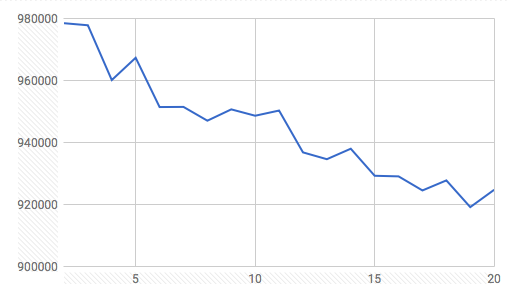
\includegraphics[width=0.4\textwidth]{pics/graph_inertia_all}
	\caption{Cost (inertia) of mini batch KMeans vs value of K\label{fig:graph_inertia_all}}   
\end{center} 
\end{figure}   

Analyzing the Figure ~\ref{fig:graph_inertia_all}, it can be seen that the smallest cost was achieved with K = $19$, so that number was utilized to perform the final clustering process and the analysis of each one's content.

To analyze the results, all headlines assigned to each cluster were separated in lists. From those headlines, its word-level 1-grams were extracted and put in order of occurrences, so the key words for each cluster could be easily assessed and consequently, the cluster's topic found.

The majority of the clusters showed headlines with high frequencies of 1-grams that led to certain closed topics. The classifications made by analyzing those terms, for all clusters, are the following:

\begin{itemize}
	\item Cluster 1: Not identified
	\item Cluster 2: Business subjects, with worlds like: business, market, nation, law, analysis
	\item Cluster 3: Disasters, with words like: crash, fear, fire
	\item Cluster 4: Elections and politics subjects, with words like: election, selection, government, poll, nation
	\item Cluster 5: International and world subjects, with words like: Australia, China, India, US, world, England
	\item Cluster 6: Police and criminality subjects, with words like: police, fatal, fire, crash, stab, theft, death
	\item Cluster 7: Disasters, tragedies and criminal subjects, with words like: police, hit, kill, die, fire, hospital
	\item Cluster 8: Work and jobs subjects, with words like: miner, coal, jobs, industries, worker
	\item Cluster 9: Not identified
	\item Cluster 10: Police, charges, criminality subjects, with words like: police, charge, fire, kill, death, crash, murder
	\item Cluster 11: Refugees, with words like: seek, seeker, asylum, help, government, support
	\item Cluster 12: Not identified
	\item Cluster 13: Criminality, with words like: arrest, robbery
	\item Cluster 14: Health, with words like: fund, health, mental, body
	\item Cluster 15: Law, with words like: trial, murder, stand, accused, charged, court
	\item Cluster 16: Politics, with words like: council, councillor, plan, mayor, government
	\item Cluster 17: Attacks (supposedly from animals) and criminality, with words like: attack, police, kill, shark, dog, woman, jail, victim
	\item Cluster 18: Television, broadcasting, TV shows, with words like: report, sport, ABC, urgent, live, rural
	\item Cluster 19: Empty cluster
\end{itemize}

After the whole cluster analysis considering the whole dataset, headlines from 3 distinct years were utilized to perform clustering in order to compare the results. The chosen years were: 2003, 2005 and 2007.

For the year 2003, the number of clusters K that showed minimal inertia was $14$, for the year 2005, $15$ and for 2007, $19$. Analyzing those numbers, it can be seen that two of them (K = $14$, for 2003, and K = $15$, for 2005) were different from the one found with all the headlines (K = $19$), and one was exactly the same (K = $19$ for 2007).

The most frequent themes that could be identified from the 2003 headlines were: criminal, law, world news, places, health, Tasmania, interviews and leadership. For the year 2005, XXX and XXX, and for 2013, XXXX.


\section{Discussion}
%%%Talk about the experiments carried out and the obtained results. 

As all methods for feature extraction were used in the literature with success, at least a good result using them was expected. 

When utilizing a feature set with features only sourced from the Local Binary Patterns, the best classifier accuracy obtained was of $38.8\%$ when utilizing logistic regression for the test set and $72\%$ for cross-validation, which may characterize overfitting.

As more features were added to try to improve the results, an unexpected drop in accuracy was shown: for logistic regression classifier, a test set accuracy of $12.2\%$ and a cross-validation accuracy of $52.2\%$ were obtained and for the neural network implementation, $16.3\%$ and $30.4\%$ respectively.
   
None of the results obtained were satisfying to classify the images correctly. Even with a $72\%$ cross-validation accuracy for the Local Binary Patterns, the classifier fell short when the input was an image from the test set.

As adding more features shown a big drop in accuracy, which in this case is counter-intuitive, either those features didn't have an effect to characterizing the sensor noise patterns or some error occurred in the algorithm implementations.

%%% Add section %%%%%%%%%%%%%%%%%%%%%%%%%%%%%%%%%%%%%%%%%%%%%%%%%%%%%%%%%%%%%%%%%%
\section{Conclusions}

After utilizing different methods with different feature sets, the final classification accuracies for the test set were far from great.

For the Linear Binary Patterns features, as it shown the best result, maybe an improvement in the post-processing of the PRNU-based noise image was needed for a more relevant result. 

For both the Linear Binary Patterns features and, after, the more complete feature set including values of mean, variance, skewness, kurtosis and correlations, there may be occurred a slight overfit, as there is a considerable difference between the cross-validation and test set accuracies. Another important detail is that probably there was a a difficulty for the classifier to identify modified pictures (as it happens in half of the pictures from the test set), aggravated by the fact that the correlations between the noise of the image being analyzed and the means of the noises from all pictures for each camera were taken considering only a central patch of $512$ by $512$ pixels, which probably led to values that weren't "assertive" enough to weight in the classification process.
 
%%% References %%%%%%%%%%%%%%%%%%%%%%%%%%%%%%%%%%%%%%%%%%%%%%%%%%%%%%%%%%%%%%%%%%%
\section{References}

[1] Jocelin Rosales Corripio and David Maniel Arenas Gonzalez and Ana Lucila Sandoval Orozco and Luis Javier Garcia Villalba and Julio Hernandez-Castro and Stuart James Gibson. Source Smarphone Identification Using Sensor Pattern Noise and Wavelet Transform. In \textit{Proceedings of the IEEE Computer Society Conference on Computer Vision and Pattern Recognition (CVPR)}, London, UK, 2013.

[2] Guansho Xu and Yun Qing Shi. Camera Model Identification Using Local Binary Patterns. In \textit{Imaging for Crime Detection and Prevention, 2013, ICDP.}, Melbourne, Australia, 2012.


\end{document}